\chapter{Data model}

The \acrshort{gsdm} implements the data model shown in the figure \ref{fg:gsdmdb}.

\begin{figure}[ht]
  \begin{center}
	\centering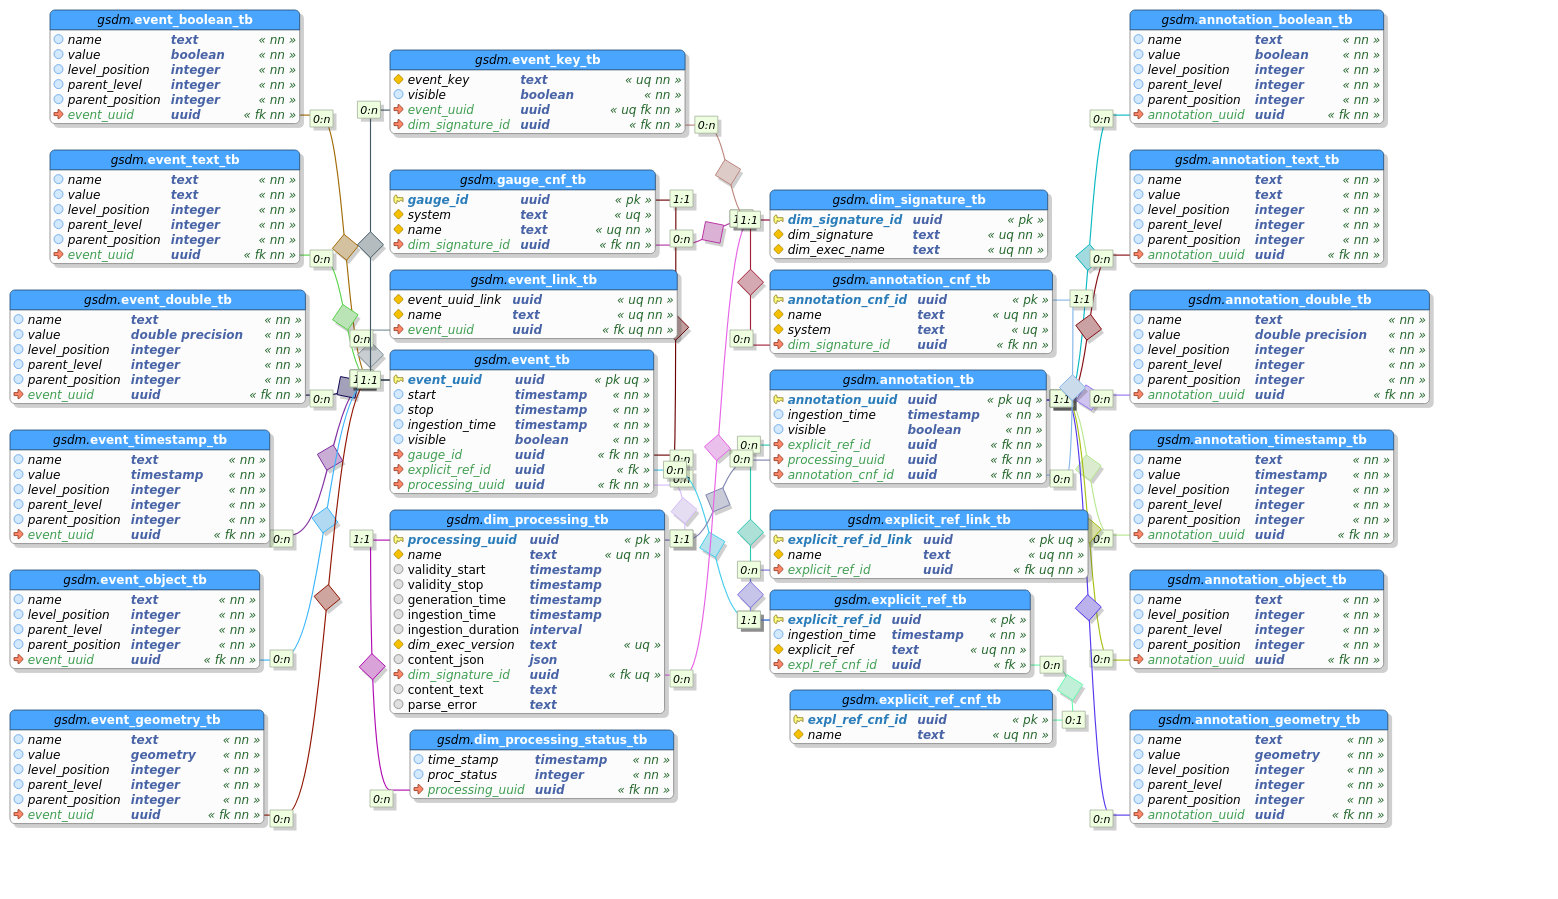
\includegraphics[width=150mm]{../fig/gsdmdb.png}
	\caption{Data model of the \acrshort{gsdm}}
	\label{fg:gsdmdb}
  \end{center}
\end{figure}

As said in chapter \ref{c:intro}, there are 4 main entities in the data model: explicit references (explicit\_ref\_tb), events (event\_tb), annotations (annotation\_tb) and inputs (dim\_processing\_tb).

The entities event and annotation may have an associated dynamic structure of values. These values indicate properties/information of the related entities interesting for the data model. These values are structured in the database following the schema of the figure \ref{fg:values_structure}.

\begin{figure}[ht]
  \begin{center}
	\centering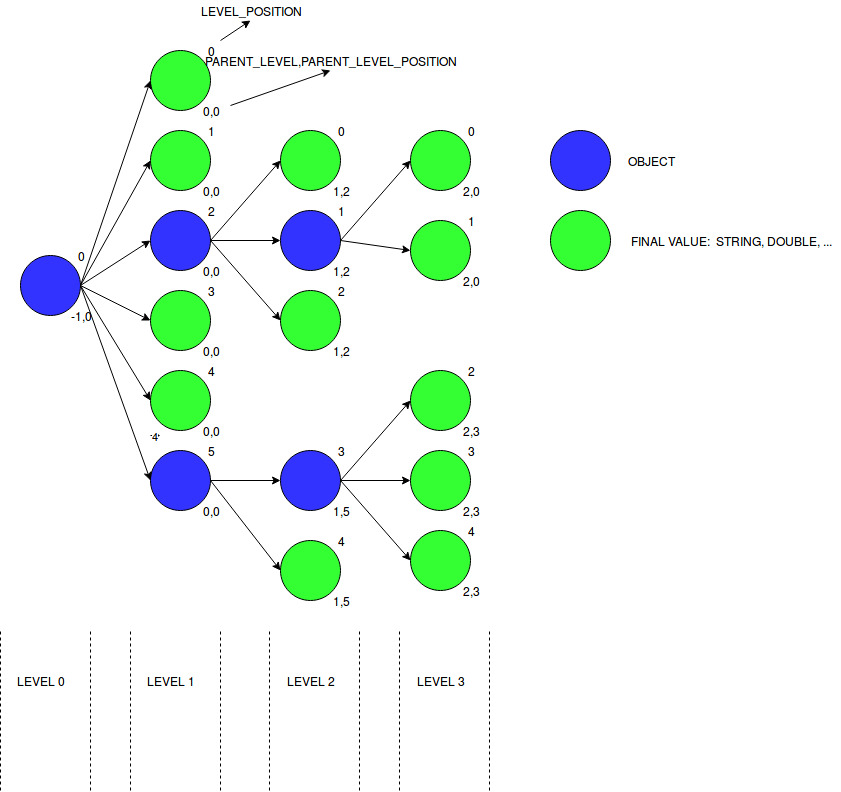
\includegraphics[width=150mm]{../fig/values_structure.jpg}
	\caption{Structure of the values associated to events and annotations}
	\label{fg:values_structure}
  \end{center}
\end{figure}

The values associated to an entity may have one of the following types:

\begin{itemize}

\item Boolean
\item Text
\item Double
\item Timestamp
\item Geometry
\item Object

\end{itemize}

The type object allows every entity to have an associated structure of values (containing other objects). This structure is defined like a tree, every node of the tree may have any of the types described in the previous list. If the node has the type object, the branch has to continue till the final node has a type different than the type object.
The way the tree is structured is as follows:

\begin{enumerate}

\item Every node has a level position
\item Every node has a reference to its parent represented by the parent level and parent level position values
\item Every parent node has the type object
\item Every final node of a branch has a type different than the type object

\end{enumerate}

To better understand how the structure of values is managed by the \acrshort{gsdm}, here it is an example:

Input:
\begin{lstlisting}[breaklines=true, style=xml, caption={XML input example for showing the values structure management.}]
<gsd>
  <insert>
    <dim_signature
        name="test_dim_signature1"
        version="1.0"
        exec="test_exec1"/>
    <source
        name="test_simple_update.xml" 
        generation_time="2018-06-06T13:33:29"
        validity_start="2018-06-05T02:07:03"
        validity_stop="2018-06-05T02:07:36"/>
    <data>
      <event start="2018-06-05T02:07:03"
             stop="2018-06-05T02:07:36"
             key="test_key2"
             explicit_reference="test_explicit_ref2"
             link_ref="event_link_id2">
        <links>
          <link name="test_link_name2" link_mode="by_ref">event_link_id1</link>
        </links>
        <gauge name="test_gauge_name2"
               system="test_gauge_system2"
               insertion_type="SIMPLE_UPDATE"/>
        <values name="test_object_name2">
          <value name="test_text_name2" type="text">test text2</value>
          <value name="test_boolean_name2" type="boolean">true</value>
          <value name="test_double_name2" type="double">0.91234</value>
          <values name="test_object_name3">
            <value name="test_text_name3" type="text">test text2</value>
            <value name="test_geometry2" type="geometry">29.012974905944
            -118.33483458667
            29.012974905944
            -118.33483458667</value>
          </values>
        </values>
      </event>
    </data>
  </insert>
</gsd>
\end{lstlisting}

Output:

\begin{lstlisting}[breaklines=true, caption={JSON output after query the gsdm for the specific event previously shown.}]

{"_sa_instance_state": <sqlalchemy.orm.state.InstanceState object at 0x7f633a920630>,
 "event_uuid": UUID("b271b268-b048-11e8-b1cd-000000006318"),
 "level_position": 0,
 "name": "test_object_name2",
 "parent_level": -1,
 "parent_position": 0}
{"_sa_instance_state": <sqlalchemy.orm.state.InstanceState object at 0x7f633a9304e0>,
 "event_uuid": UUID("b271b268-b048-11e8-b1cd-000000006318"),
 "level_position": 0,
 "name": "test_text_name2",
 "parent_level": 0,
 "parent_position": 0,
 "value": "test text2"}
 {"_sa_instance_state": <sqlalchemy.orm.state.InstanceState object at 0x7f633a9306d8>,
 "event_uuid": UUID("b271b268-b048-11e8-b1cd-000000006318"),
 "level_position": 1,
 "name": "test_boolean_name2",
 "parent_level": 0,
 "parent_position": 0,
 "value": True}
 {"_sa_instance_state": <sqlalchemy.orm.state.InstanceState object at 0x7f633a92b0b8>,
 "event_uuid": UUID("b271b268-b048-11e8-b1cd-000000006318"),
 "level_position": 2,
 "name": "test_double_name2",
 "parent_level": 0,
 "parent_position": 0,
 "value": 0.91234}
 {"_sa_instance_state": <sqlalchemy.orm.state.InstanceState object at 0x7f633a920f60>,
 "event_uuid": UUID("b271b268-b048-11e8-b1cd-000000006318"),
 "level_position": 3,
 "name": "test_object_name3",
 "parent_level": 0,
 "parent_position": 0}
{"_sa_instance_state": <sqlalchemy.orm.state.InstanceState object at 0x7f633a930550>,
 "event_uuid": UUID("b271b268-b048-11e8-b1cd-000000006318"),
 "level_position": 0,
 "name": "test_text_name3",
 "parent_level": 1,
 "parent_position": 3,
 "value": "test text2"}
{"_sa_instance_state": <sqlalchemy.orm.state.InstanceState object at 0x7f633a9303c8>,
 "event_uuid": UUID("b271b268-b048-11e8-b1cd-000000006318"),
 "level_position": 1,
 "name": "test_geometry2",
 "parent_level": 1,
 "parent_position": 3,
 "value": <WKBElement at 0x7f633a9305f8; 01030000000100000037000000bab2cc5252033d404fd40bee6d955dc0b71be99d72dd3c40e4ff1f50cf975dc03fd8f5e298b73c4015a6d00c2f9a5dc00b173561be913c40117082478d9c5dc0142857d6e06b3c40edf52a6fea9e5dc0759e911afe453c40e7807a3247a15dc00b99eda117203c4054bc9b6da3a35dc08e6c65542dfa3b4086b0ab05ffa55dc00fec708441d43b401f266aa959a85dc0c234706521c13b409a546f4e89a95dc02b2990c36dba3b4073ad4aa9bd9e5dc0ef04fb9096b33b40c10d6c571b945dc0a31409a298ac3b40741fa9a29d895dc041ca98b770a53b40f95e32e53f7f5dc04f61ea7e1b9e3b40e3646887fd745dc0f99a399195963b401afbb3fdd16a5dc07c744273db8e3b40382a94c6b8605dc078708094e9863b40816ea968ad565dc0a385764ebc7e3b40d9a80b71ab4c5dc0b04095e34f763b40f7037e71ae425dc01432147ea06d3b4090abc8feb1385dc0f4567d2eaa643b409a170bafb12e5dc0a77c05ea685b3b407b040b18a9245dc092cdc288d8513b40e8ada7cd931a5dc0470088c3f4473b40207f1e606d105dc0606fa831b93d3b40ed827d5a31065dc0e463305321333b404a701f4fdbfb5cc083263eed09273b40166ec11359f05cc04b4176f41e3a3b40edb9b49509ef5cc06ac2ec29f55f3b404c4c24666fec5cc05706f32bc9853b40b5087efcd3e95cc00df5b35597ab3b407c3bfe7737e75cc0e835fedc5fd13b40b92260099ae45cc0f5bb443821f73b403d9452eafbe15cc01b27e9d6dd1c3c403529415a5cdf5cc0028b00fe98423c40975de8d3badc5cc0421be70d5c683c40f30d99ef16da5cc0dd840c8587743c4019d72226bae55cc05b2b8ebc307f3c4073d37b012ef05cc00de2d1c87c893c406f20bea487fa5cc0860fb83b70933c40ee7aeb8ecb045dc00e0d1f9b0f9d3c401d362657fe0e5dc08533ac295fa63c40f0a9496824195dc0d196c11763af3c403ade713a42235dc0171a48771fb83c40de6ab2435c2d5dc0637dc83d98c03c40423d0cfa76375dc00854fc45d1c83c4016f2f5d496415dc060e03f51ced03c408b34164fc04b5dc075a9d20893d83c40d4d6fee7f7555dc01c75cafe22e03c402000de2542605dc086b7ecae81e73c4027645297a36a5dc0dd0f407fb2ee3c408cb137d520755dc0f2359ec0b8f53c40fbecc084be7f5dc05ad5879397fc3c40d08b3635818a5dc0bab2cc5252033d404fd40bee6d955dc0>}
 
\end{lstlisting}

So, all values are associated to the proper level position, parent level and parent level position values.